\section{Introduction}
\label{s:Introduction}

We want to build a wireless sensors network for performance analysis. The final goal is to have different kinds of sensors connected together and to be able to visualize measurements and to configure them from a GUI.

\begin{figure}[ht]
\centering
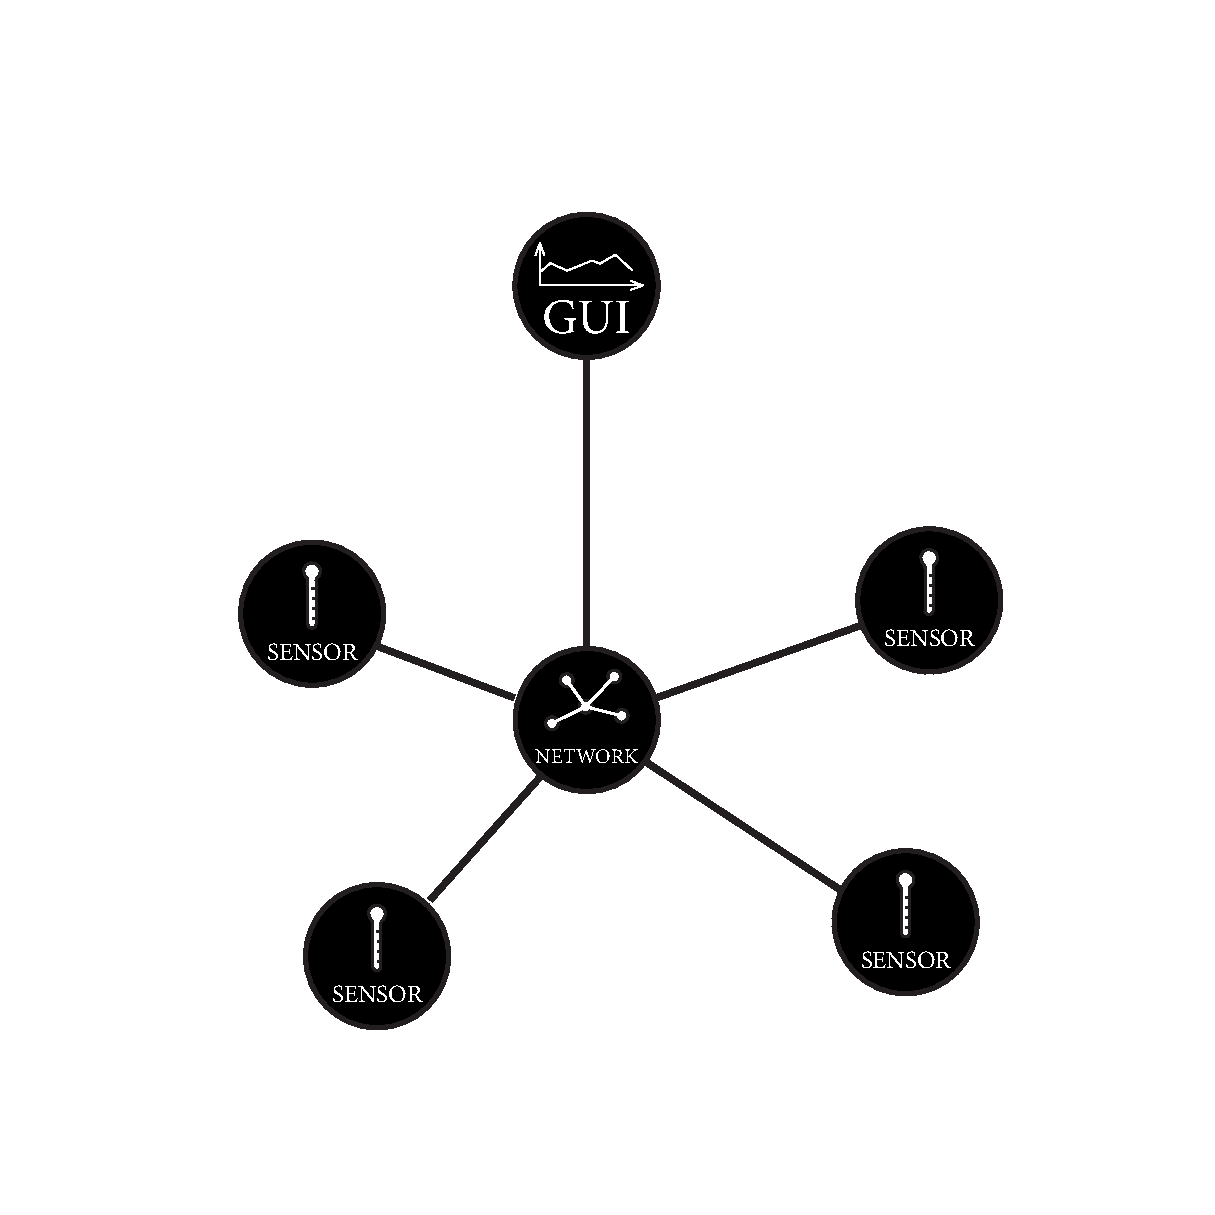
\includegraphics[width=.6\linewidth]{global_archi}
\caption[General Architecture]{\label{f:global_archi}General architecture.}
\end{figure}

To begin with, wireless communication protocols are explored. Once one is chosen and a hardware implementation is picked, we start exploring the system and show that drivers for peripherals can easily be written. Next, we continue with the interesting part of the system, the communications, and we finish by a method to share a common time among all nodes of the network.

All our work is available on our github : \url{https://github.com/Aunsiels/Mesh_Bee}